\documentclass[conference]{IEEEtran}
\usepackage[utf8]{inputenc}
\usepackage[brazilian,provide=*]{babel}
\usepackage{amsmath,booktabs,graphicx}
\usepackage[hidelinks]{hyperref}
\graphicspath{{../resultados/}}
\renewcommand{\abstractname}{Resumo}
\renewcommand{\IEEEkeywordsname}{Palavras-chave}
\title{Análise Computacional de Estabilidade pelo Critério de Nyquist em Sistemas com e sem Atraso}
\author{\IEEEauthorblockN{Thiago Henrique e Mateus Afonso}
\IEEEauthorblockA{Engenharia de Computação\\Pontifícia Universidade Católica de Goiás}}
\begin{document}
\maketitle
\begin{abstract}
Este trabalho compara Nyquist, Routh--Hurwitz, lugar das raízes e Bode em quatro malhas lineares. Em uma malha com atraso de 1,35\,s, Nyquist detectou dois polos de malha fechada no semiplano direito, enquanto Padé de primeira ordem indicou estabilidade. O atraso crítico contínuo foi $1{,}325818$\,s e o modelo amostrado a 50\,Hz forneceu $1{,}305142$\,s. Para ordens 5, 10 e 20, Routh teve o menor tempo de CPU nas cargas medidas. Em polinômios com raízes repetidas, o erro direto nos polos cresceu com a ordem mesmo com resíduos pequenos.
\end{abstract}
\begin{IEEEkeywords}
Nyquist, estabilidade, atraso de transporte, Padé, PID, ESP32.
\end{IEEEkeywords}

\section{Introdução}
Atrasos de comunicação consomem margem de fase e podem desestabilizar uma malha. A atividade \cite{aed} propõe comparar quatro métodos de estabilidade e aplicar os resultados a uma bancada de controle. Foram estudadas malhas SISO contínuas, lineares, estritamente próprias, de coeficientes reais e com realimentação negativa unitária, em representações sem cancelamentos instáveis.

\section{Fundamentação teórica}
\subsection{Mapeamento conforme e princípio do argumento}
Para $L(s)=G(s)H(s)$, define-se $F(s)=1+L(s)$. Fora de polos e pontos com derivada nula, uma função analítica com derivada não nula preserva ângulos localmente. O princípio do argumento, por sua vez, relaciona a variação total de fase ao número de zeros e polos internos. Percorre-se o eixo imaginário de $-jR$ a $+jR$ e fecha-se pelo arco direito em sentido horário. A translação $F=1+L$ corresponde a observar $L$ em torno de $-1+j0$. Assim,
\begin{equation}
 N=-\frac{\Delta\arg F}{2\pi},\qquad Z=P+N ,
\end{equation}
em que $P$ conta polos abertos no semiplano direito, $Z$ conta polos fechados nesse semiplano e $N$ conta voltas horárias líquidas. Desvios à direita excluem os polos abertos sobre o eixo. Se $F(j\omega)=0$, há polo fechado na fronteira e a contagem ordinária não se aplica diretamente \cite{astrom}.

\subsection{Margens, atraso e Padé}
Em $\omega_g$, $|L(j\omega_g)|=1$ e $\mathrm{MF}=180^\circ+\angle L(j\omega_g)$, com fase referida ao cruzamento crítico. Em $\omega_f$, $L(j\omega_f)$ é real negativo e $\mathrm{MG}=-20\log_{10}|L(j\omega_f)|$. Cruzamentos múltiplos e malhas abertas instáveis exigem interpretar as margens em conjunto com a contagem de Nyquist \cite{astrom}.

O fator $e^{-\tau s}$ tem módulo unitário em $s=j\omega$ e acrescenta fase $-\omega\tau$ rad. Padé diagonal substitui o fator por $Q_m(-\tau s)/Q_m(\tau s)$, onde
\begin{equation}
 Q_m(x)=\sum_{k=0}^{m}\frac{(2m-k)!\,m!}{(2m)!\,k!\,(m-k)!}x^k .
\end{equation}
Para $m=1$, obtém-se $(1-\tau s/2)/(1+\tau s/2)$. A magnitude é preservada no eixo imaginário, mas a fase é aproximada \cite{pade}.

\subsection{Métodos comparativos}
Routh--Hurwitz organiza coeficientes alternados nas duas primeiras linhas. Para linhas consecutivas $a,b$, a linha seguinte tem elementos $a_{j+1}-a_0b_{j+1}/b_0$. Trocas de sinal na primeira coluna contam raízes à direita. Pivô nulo em linha não nula usa $\varepsilon\to0^+$ e linha nula usa a derivada do polinômio auxiliar da linha superior. Raízes sobre o eixo exigem análise adicional. O lugar das raízes acompanha os polos de $D(s)+KN(s)=0$ conforme $K$ varia. Bode representa ganho em decibéis e fase em graus contra frequência logarítmica \cite{astrom,ogata}.

\section{Plantas e implementação}
A Tabela~\ref{tab:modelos} define as plantas. O ganho $K$ multiplica o numerador indicado e vale 1 no ponto nominal.
\begin{table}[htbp]
\caption{Malhas de teste e equações características nominais}
\label{tab:modelos}
\centering\small
\begin{tabular}{@{}cll@{}}
\toprule
Caso & $L(s)$ & Equação característica\\
\midrule
A & $\frac{12}{(s+1)(s+2)(s+3)}$ & $s^3+6s^2+11s+18=0$\\[4pt]
B & $\frac{3}{(s-1)(s+2)}$ & $s^2+s+1=0$\\[4pt]
C & $\frac{1{,}5(1-s)}{(s+1)^2}$ & $s^2+0{,}5s+2{,}5=0$\\[4pt]
D & $\frac{\sqrt{17}e^{-\tau s}}{s(s+4)}$ & $s(s+4)+\sqrt{17}e^{-\tau s}=0$\\
\bottomrule
\end{tabular}
\end{table}

O núcleo usa Python e NumPy. Uma desigualdade triangular nos coeficientes garante $|L(s)|<0{,}05$ no arco externo. O programa concentra amostras perto dos desvios e cruzamentos de ganho e soma
\begin{equation}
 -\frac{1}{2\pi}\sum_{k=0}^{M-1}
 \arg\!\left(\frac{F(s_{k+1})}{F(s_k)}\right),\qquad s_M=s_0 .
\end{equation}
Aceita-se um inteiro após três refinamentos coerentes, passos menores que $\pi/3$ e distância mínima acima da tolerância. A saída pode ser inconclusiva. A resolução do contorno e o condicionamento das raízes limitam o diagnóstico numérico.

Os cruzamentos de ganho são raízes positivas de $|D(j\omega)|^2-|N(j\omega)|^2=0$ em $\omega^2$. Para malhas racionais, a fase crítica vem de $\Im[N(j\omega)D(-j\omega)]=0$ com parte real negativa. Com atraso, emprega-se varredura em faixa finita e bisseção. Routh normaliza linhas por fatores positivos e usa $\varepsilon=10^{-9}$. O lugar das raízes calcula as raízes a cada ganho e liga os pontos por proximidade, com ambiguidade em raízes múltiplas. SciPy foi reservado para validação cruzada, degraus e discretização \cite{scipy}.

\section{Validação nos quatro sistemas}
\begin{table}[htbp]
\caption{Contagens, margens e polos em $K=1$}
\label{tab:valid}
\centering\small
\begin{tabular}{@{}crrrrrr@{}}
\toprule
Caso & $P$ & $N$ & $Z$ & MG (dB) & MF ($^\circ$) & $\max\Re(s)$\\
\midrule
A &0&0&0&13,98&75,64&$-0{,}783$\\
B &1&$-1$&0&$-3{,}52$&17,94&$-0{,}500$\\
C &0&0&0&2,50&35,43&$-0{,}250$\\
D &0&2&2&$-0{,}14$&$-1{,}39$&$+0{,}00704$\\
\bottomrule
\end{tabular}\\
\footnotesize Em D, $\tau=1{,}35$\,s e a raiz foi calculada com o exponencial.
\end{table}

\textbf{A.} A primeira coluna de Routh é $1,6,8,18$. Para ganho variável, a linha $s$ contém $[66-(6+12K)]/6=10-2K$. Portanto, entre ganhos positivos, $0<K<5$ dá estabilidade. Em $\omega_f=\sqrt{11}$, o denominador aberto vale $-60$, logo $\mathrm{MG}=20\log_{10}(5)=13{,}98$\,dB. Os polos são aproximadamente $-4{,}435$ e $-0{,}783\pm j1{,}856$.

\textbf{B.} Os polos abertos são $+1$ e $-2$. Uma volta anti-horária dá $N=-1$ e $Z=1-1=0$. O polinômio $s^2+s+3K-2$ exige $K>2/3$. Em $K=1$, os polos são $-0{,}5\pm j\sqrt{3}/2$. Como $L(0)=-1{,}5$, a margem em corrente contínua é $20\log_{10}(2/3)$, limite de redução de ganho.

\textbf{C.} O zero aberto é $+1$. A coluna de Routh é $1,2-1{,}5K,1+1{,}5K$, fornecendo $0<K<4/3$ para ganho positivo. Em $K=1$, os polos são $-0{,}25\pm j1{,}561$. O degrau parte com inclinação $-1{,}5$ e converge a $1{,}5/2{,}5=0{,}6$.

\textbf{D.} O integrador é excluído por um desvio à direita. A magnitude unitária exige $\omega_g^2(\omega_g^2+16)=17$, ou $(\omega_g^2-1)(\omega_g^2+17)=0$. Daí $\omega_g=1$\,rad/s. A fase é $-\pi/2-\arctan(1/4)-\tau$. O primeiro cruzamento de $-\pi$ ocorre em
\begin{equation}
 \tau_{\mathrm{cr}}=\pi/2-\arctan(1/4)=\arctan(4)
 =1{,}3258176637\ \text{s}.
\end{equation}
Para $\tau=0$, $s^2+4s+\sqrt{17}$ é estável. No cruzamento, $s=\pm j$. Derivando implicitamente $s(s+4)+\sqrt{17}e^{-\tau s}=0$, obtém-se
\begin{equation}
 \Re\frac{ds}{d\tau}=\frac{18}{(4-\tau)^2+(2+4\tau)^2}>0
 \quad\text{em }s=j .
\end{equation}
O par cruza para a direita. Em $1{,}35$\,s, a raiz superior localizada por SciPy foi $0{,}007036+j0{,}989491$, com resíduo de $7{,}11\times10^{-16}$. Nyquist forneceu $P=0,N=2,Z=2$. Em A--C, a contagem coincidiu com Routh e com os autovalores da matriz companheira. O erro máximo da resposta em frequência contra SciPy foi $1{,}16\times10^{-15}$ na grade usada.

\begin{figure}[htbp]
\centering
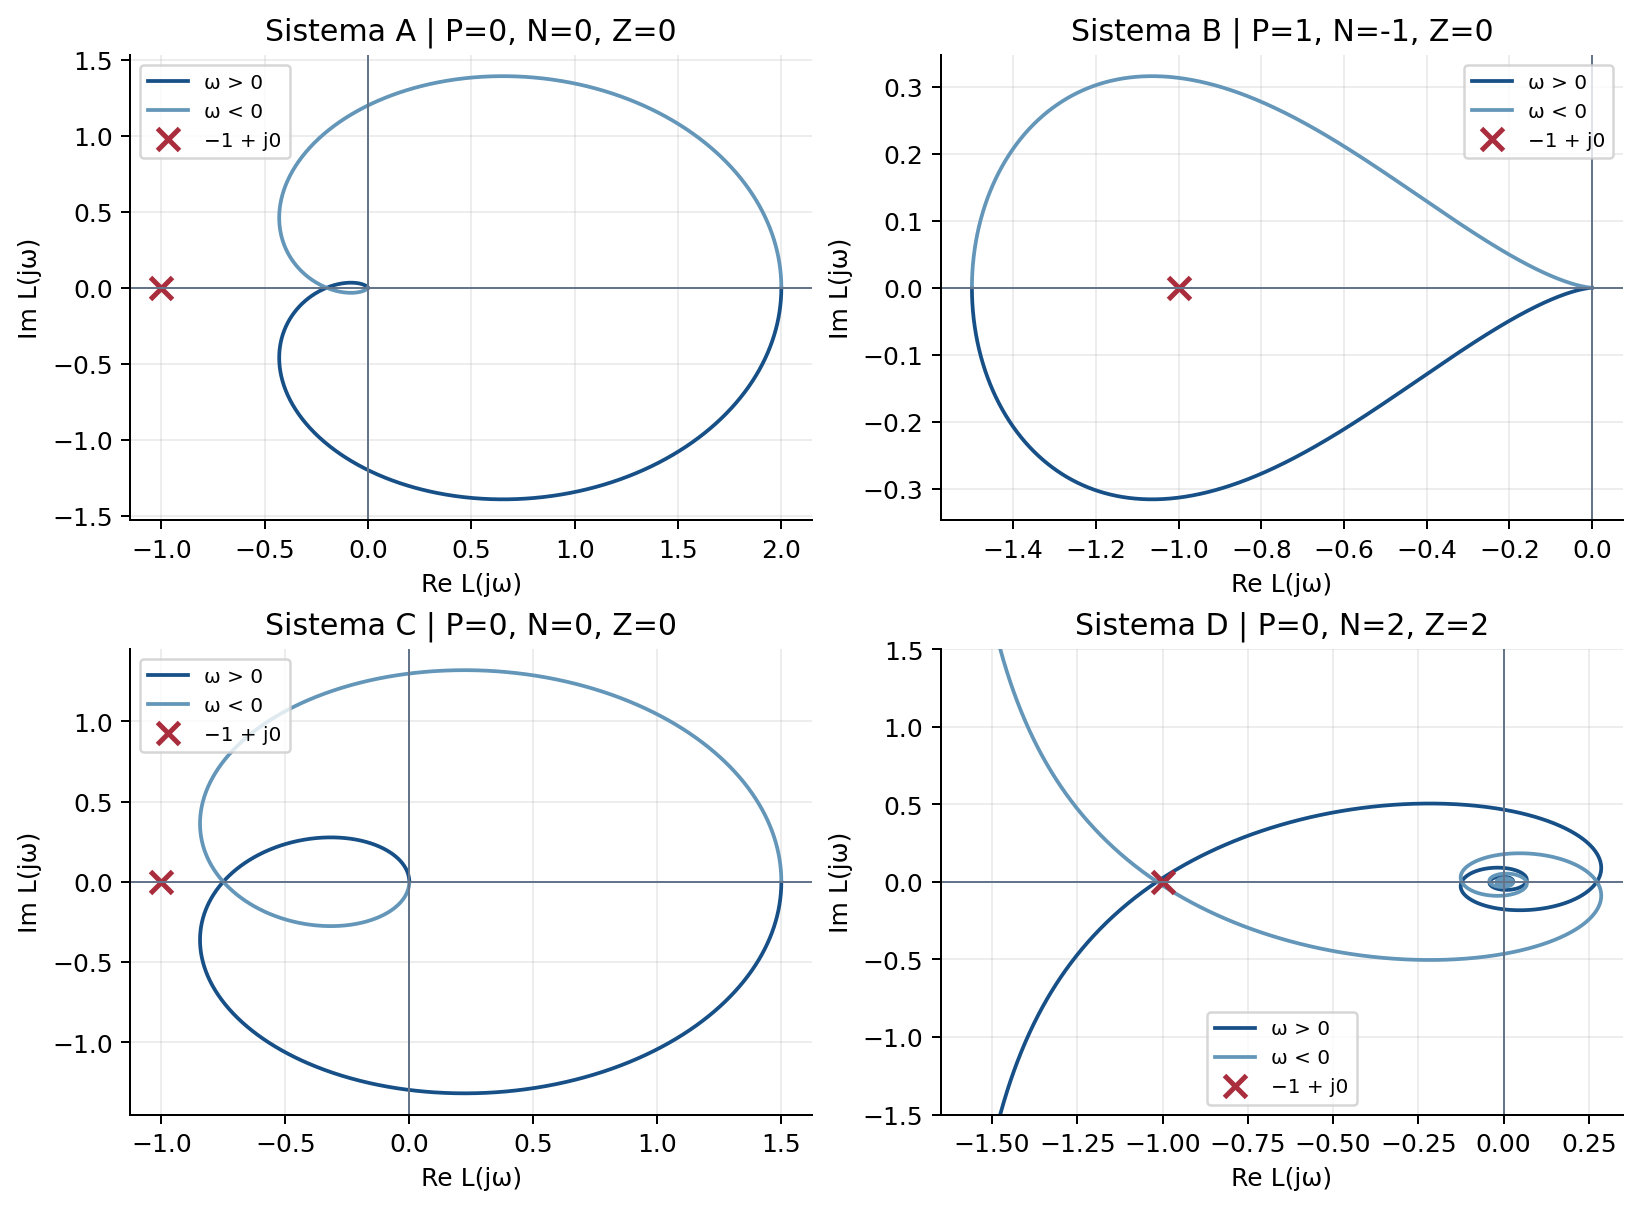
\includegraphics[width=\columnwidth]{nyquist.png}
\caption{Ramos em frequência. Em D, ampliação perto do ponto crítico. A contagem usa o contorno fechado, incluindo o desvio em D.}
\end{figure}

\section{Atraso exato e aproximações}
Em Padé $[1/1]$, a fase adicional é $-2\arctan(\tau/2)$ no cruzamento de ganho. Igualando a perda de fase a $\arctan(4)$, resulta $\tau_{\mathrm{cr},[1/1]}=2\tan(\arctan(4)/2)=1{,}5615528128$\,s. O erro relativo é $100(\tau_{\mathrm{Pade}}-\tau_{\mathrm{cr}})/\tau_{\mathrm{cr}}$. Em 1,35\,s, Padé $[1/1]$ tem MF $+7{,}93^\circ$ e zero trocas em Routh. O modelo exato tem MF $-1{,}39^\circ$ e dois polos instáveis.
\begin{table}[htbp]
\caption{Limiar de atraso e polos instáveis em $\tau=1{,}35$\,s}
\centering\small
\begin{tabular}{@{}lrrr@{}}
\toprule
Modelo & Limiar (s) & Erro (\%) & Polos instáveis\\
\midrule
Exato & 1,325817664 & 0 & 2\\
$[1/1]$ & 1,561552813 & 17,78036 & 0\\
$[2/2]$ & 1,331015330 & 0,39203 & 2\\
$[3/3]$ & 1,325884353 & 0,00503 & 2\\
$[4/4]$ & 1,325818137 & 0,00004 & 2\\
\bottomrule
\end{tabular}
\end{table}
\begin{figure}[htbp]
\centering
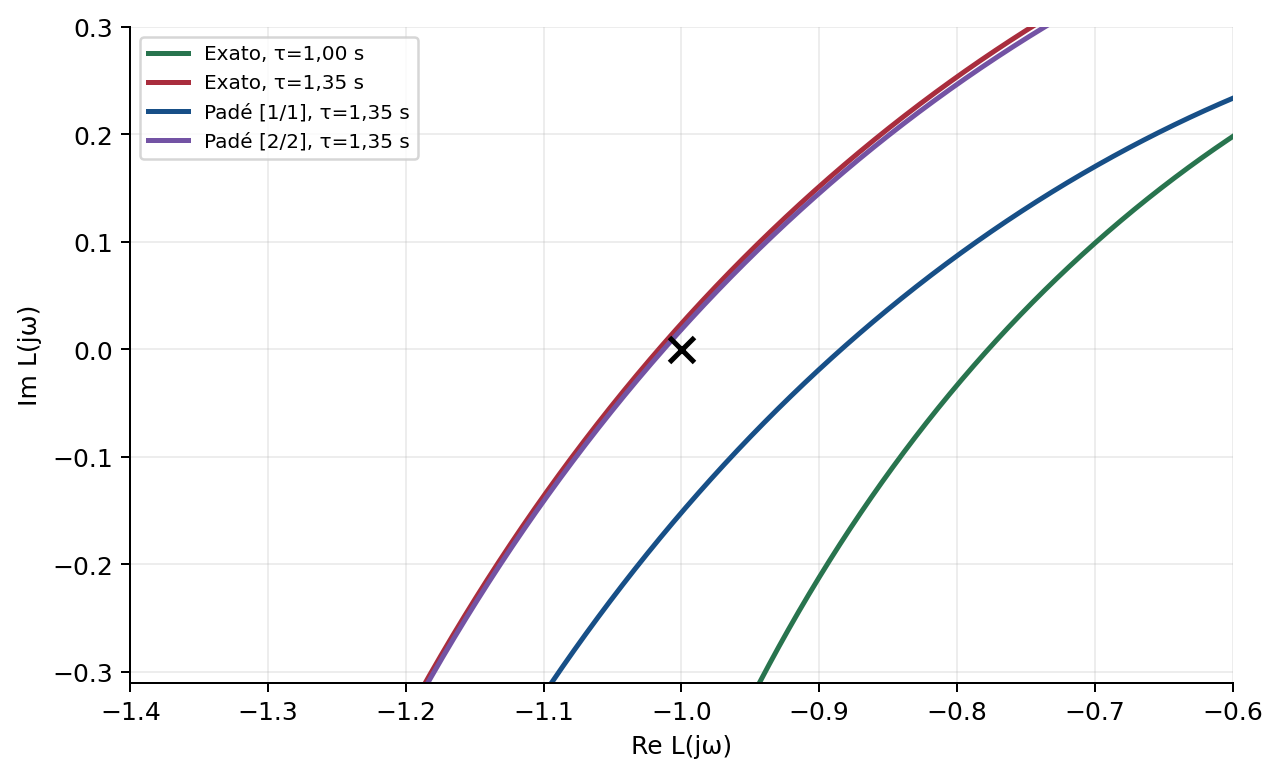
\includegraphics[width=\columnwidth]{atraso_pade.png}
\caption{Comparação perto de $-1+j0$ no ramo $\omega>0$.}
\end{figure}

\section{Custo e arredondamento}
Para $n=5,10,20$, avaliou-se $L_n(s)=0{,}25/((s+1)^n-0{,}25)$. Em $K=1$, o polinômio fechado é $(s+1)^n$. Usaram-se quatro aquecimentos e 25 medições de CPU por configuração, 4096 frequências para Bode e 301 ganhos para o lugar das raízes. As medições excluem gráficos e arquivos. O ambiente reportou AMD EPYC 9V45, Linux x86-64, Python 3.12.14, NumPy 2.3.5 e SciPy 1.17.0.
\begin{table}[htbp]
\caption{Mediana de CPU em microssegundos}
\centering\small
\begin{tabular}{@{}lrrr@{}}
\toprule
Método & $n=5$ & $n=10$ & $n=20$\\
\midrule
Routh &31,0&58,0&118,1\\
Nyquist &523,3&583,5&738,8\\
Bode com margens &168,2&234,5&460,7\\
Lugar das raízes &8635,0&14620,1&29337,6\\
\bottomrule
\end{tabular}
\end{table}

Routh monta $\mathcal O(n^2)$ entradas. Avaliar $M$ frequências por Horner custa $\mathcal O(Mn)$, além dos cálculos de cruzamentos e refinamento. O lugar das raízes repete a solução por autovalores a cada ganho, com associação gulosa de custo cúbico por passo no pior caso \cite{numpy}. Os tempos correspondem às cargas e grades escolhidas.

O erro direto máximo, $\max_i|\hat p_i+1|$, foi $9{,}53\times10^{-4}$, $5{,}13\times10^{-2}$ e $3{,}95\times10^{-1}$ para $n=5,10,20$. O resíduo relativo máximo $|p(\hat p_i)|/\sum_k|a_k||\hat p_i|^{n-k}$ ficou abaixo de $2{,}32\times10^{-16}$. A maior diferença entre as tabelas normalizadas de Routh em float32 e float64 cresceu de $3{,}58\times10^{-8}$ para $2{,}99\times10^{-6}$, com zero trocas em ambas. O uso deliberado de raízes repetidas ilustra seu mau condicionamento \cite{numpy}.

\section{Demonstração em Engenharia de Computação}
A planta simulada é $G_p(s)=1/(s+1)^2$. O PID filtrado usa
\begin{align}
 C(s)&=K_p+K_i/s+K_d s/(1+s/4),\\
 (K_p,K_i,K_d)&=\sqrt{17}(7/16,1/4,9/64).
\end{align}
Agrupar o controlador dá $\sqrt{17}(s+1)^2/[s(s+4)]$. Os dois cancelamentos estáveis dão a malha D. A bancada discretiza o PID por Euler para trás com $T_s=20$\,ms e atualiza a planta por retenção de ordem zero. Com $a=e^{-T_s}$ e $d=\mathrm{round}(\tau/T_s)$,
\begin{align}
 x_{1,k+1}&=ax_{1,k}+(1-a)u_{k-d},\\
 x_{2,k+1}&=a(x_{2,k}+T_s x_{1,k})+[1-a(1+T_s)]u_{k-d},\\
 y_k&=x_{2,k}.
\end{align}
O hospedeiro envia índice e erro $1-y_k$. O firmware devolve índice e comando pela serial a 115200\,bit/s \cite{esp}. A fila atrasa o comando. O hospedeiro registra o tempo de ida e volta e encerra o modo em tempo real se perder o prazo de amostra.

A malha discreta cruza ganho unitário em $1{,}007226$\,rad/s. Avaliar $[\pi+\angle L_d(e^{j\omega_g T_s})]/\omega_g$ dá $1{,}305142$\,s, entre 65 e 66 amostras. Executaram-se 3001 amostras por cenário com o PID C++ como processo local. A razão entre máximos de $|y-1|$ nas janelas de 50 a 60\,s e 30 a 40\,s foi $0{,}078$ em 1,00\,s, $1{,}086$ em 1,32\,s e $2{,}710$ em 1,50\,s. O firmware e o roteiro serial estão preparados. A compilação para a placa e o ensaio HIL físico permanecem pendentes.
\begin{figure}[htbp]
\centering
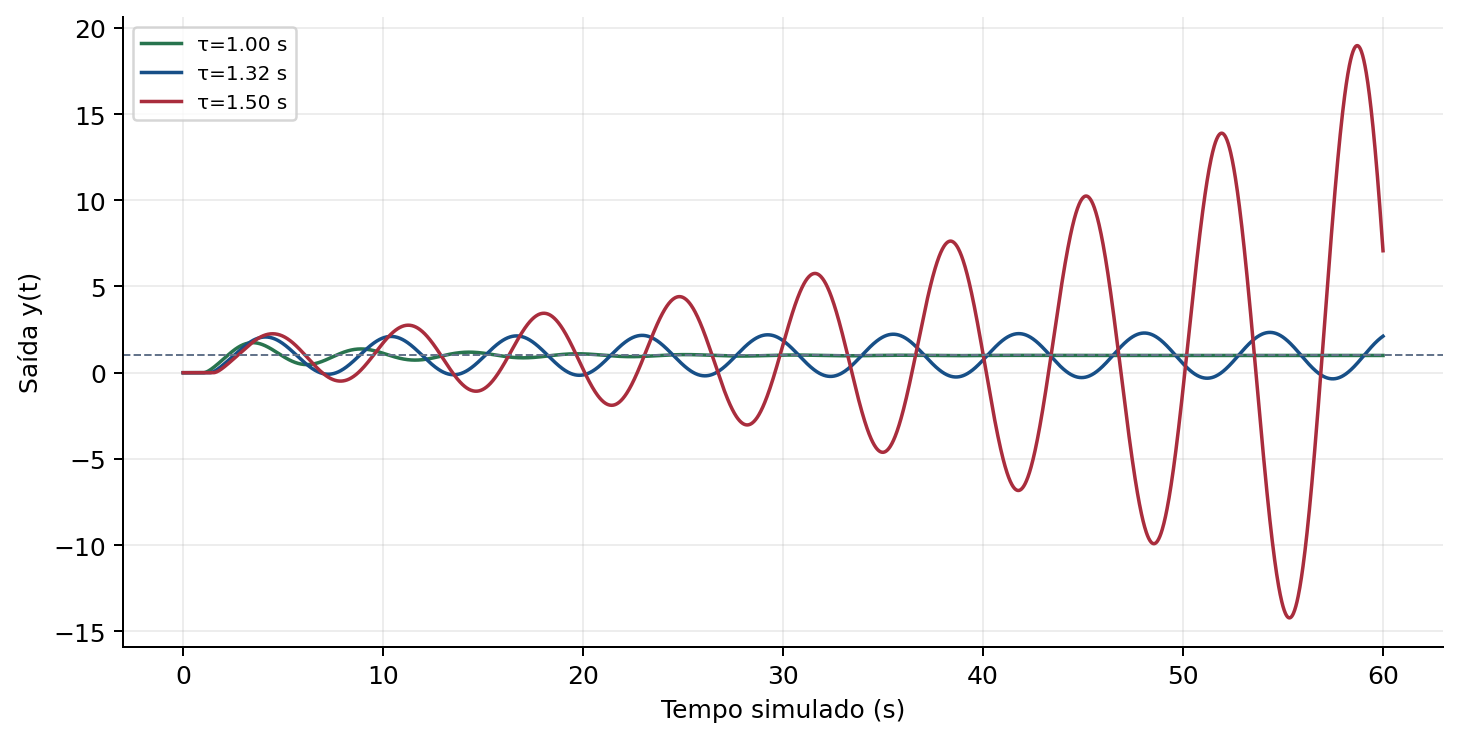
\includegraphics[width=\columnwidth]{bancada.png}
\caption{Degrau da bancada em software com PID C++ e três atrasos.}
\end{figure}

\section{Conclusão}
Nyquist, Routh e a verificação por polos concordaram para as três malhas racionais. O lugar das raízes indicou os limites de ganho. Bode forneceu margens que dependem da condição de estabilidade aberta e do sentido da perturbação. Em D, Padé de ordem 1 superestimou o atraso crítico e produziu um diagnóstico incorreto em 1,35\,s. A discretização a 50\,Hz reduziu o limiar em cerca de 20,68\,ms, pela diferença entre os limiares contínuo e discreto. O código e os dados permitem repetir a comparação e estender o experimento à placa.

\begin{thebibliography}{00}
\bibitem{aed} Enunciado da atividade, \emph{Projeto de pesquisa aplicada: análise computacional e comparativa de critérios de estabilidade em sistemas dinâmicos}, material didático, 3 p.
\bibitem{astrom} K. J. Åström e R. M. Murray, \emph{Feedback Systems: An Introduction for Scientists and Engineers}. Princeton University Press, 2008. \url{https://fbswiki.org/wiki/index.php/Frequency_Domain_Analysis}
\bibitem{ogata} K. Ogata, \emph{Engenharia de Controle Moderno}, 5.\ ed. São Paulo: Pearson, 2010.
\bibitem{pade} MathWorks, \emph{Time-Delay Approximation}. \url{https://www.mathworks.com/help/control/ug/time-delay-approximation.html}
\bibitem{scipy} SciPy, \emph{Signal processing}. \url{https://docs.scipy.org/doc/scipy/reference/signal.html}
\bibitem{numpy} NumPy, \emph{Polynomial roots}. \url{https://numpy.org/doc/stable/reference/generated/numpy.roots.html}
\bibitem{esp} Espressif Systems, \emph{Serial (UART)}, Arduino ESP32. \url{https://docs.espressif.com/projects/arduino-esp32/en/latest/api/serial.html}
\end{thebibliography}
\end{document}
